%!TEX root = uiuc_2018_invitational.tex
\begin{problem}{Kindle the Bonfire}
{stdin}{stdout}
{1 second}{}{}

\begin{wrapfigure}{r}{0.23\textwidth}
    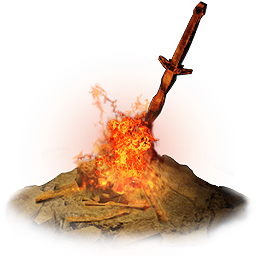
\includegraphics[scale=0.5]{bonfire.png}
\end{wrapfigure}

Being the last guardian of the lost land of Dregoheap, you are in charge 
of protecting the inhabitants in this area.

The land of Dregoheap consists of $N$ cities and $M$ roads, where each road
is bidirectional and connects exactly $2$ cities. During the day, you will
patrol around Dregoheap. When you are at some city $i$, you may receive a
distress call from some other city $j$ about an emergency event. Of course, as 
the sole guardian, you need to go to city $j$ as soon as possible  and save the
citizens there.

Luckily, at Dregoheap, there are $K$ cities which contain an unkindled bonfire.
Once a bonfire is kindled, you can teleport from that bonfire to any other 
\textit{kindled} bonfire. However, due to limited resources, you are only able 
to kindle at most $L$ bonfires.

After kindling bonfires in the optimal way,
you would like to know in the worst case, what is the longest distance you need
to travel in order to respond to one emergency event.

Note your patrol route is random, and the emergency events also happen 
randomly. You can assume traveling within a city is cost-free. Also 
teleporting between bonfires is also costfree. You will also only receive 
distress call when you are in a city, and no two emergencies events will happen
at the same time.

At last, it is guaranteed there is always a path between any pair of cities.

\InputFile

The first line of input contains two integers $N, M (1 \le N \le 20,
0 \le M \le 500)$.

In the next $M$ lines, each line will contain three integers,
$u_i, v_i, w_i$, $1 \le u_i, v_i \le N$, $1 \le w_i \le 10^6$, which means
this road connects cities $u_i, v_i$ and has length $w_i$.

The next line contains two integers $K, L (0 \le L \le K \le 10)$. 

The final line of input contains $K$ integers, denoting the indices of cities
which contain an unkindled bonfire.
\OutputFile

A single line with an integer giving the longest distance you need to travel
in case of emergency.

\Examples

\begin{example}
\exmp{
3 3
1 2 1024
1 3 1024
2 3 1024
3 3
1 3 2
}{%
0
}%
\exmp{
3 2
1 2 5
1 3 1024
3 2 
1 3 2
}{%
5
}%
\end{example}
\end{problem}
